\documentclass[letterpaper,landscape]{article}
\usepackage[margin=0.5in]{geometry}
\usepackage{array}
\usepackage{tabularx}
\usepackage{tikz}
\usepackage{amssymb}

\newcommand{\checkboxes}{
    1 \(\square\) -
    2 \(\square\) -
    3 \(\square\) -
    4 \(\square\) -
    5 \(\square\)
}
\newcommand{\row}[1]{ \rowcontent{#1}{} }
\newcommand{\rowcontent}[2]{ \rowsubtitlecontent{#1}{}{#2} }
\newcommand{\rowsubtitlecontent}[3]{ \textbf{#1} #2 & #3 & #3 & #3 & #3 & #3 }

\begin{document}

% ------------------- Front Page Grid -------------------
\noindent \parbox[t][0.3in][t]{3.5in}{\textbf{Week's Theme:}}  \textbf{Projects (max 2):} \\

\noindent \begin{tabularx}{\linewidth}{|>{\raggedleft\arraybackslash}p{0.5in}|*{5}{>{\raggedright\arraybackslash}X|}}
    \hline
    & \textbf{Monday} & \textbf{Tuesday} & \textbf{Wednesday} & \textbf{Thursday} & \textbf{Friday} \\ \hline
    \row{Focus} \\[0.8in] \hline
    \rowcontent{Work}{
        1.\par\vspace{0.5in}
        2.\par\vspace{0.5in}
        3.\par\rule{0pt}{0.5in}
    } \\ \hline
    \rowcontent{Chores}{
        4.\par\vspace{0.5in}
        5.\par\rule{0pt}{0.5in}
    } \\ \hline
    \row{Notes} \\[1.5in] \hline
    \rowsubtitlecontent{Daily}{
    work \par
    chores \par
    excersise \par
    }{
        \hspace*{-0.1in}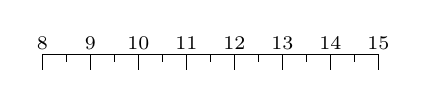
\begin{tikzpicture}[x=0.24in, every node/.style={font=\scriptsize}]
            \draw (8,0) -- (15,0);
            \foreach \x in {8,...,15}
                \draw (\x, 0) -- (\x, -0.2) node[above=4pt] {\x};
            \foreach \x in {8.5,9.5,...,14.5}
                \draw (\x, 0) -- (\x, -0.1);
        \end{tikzpicture}
    } \\[0.5in] \hline
    \rowcontent{Done}{\checkboxes} \\ \hline
\end{tabularx}

\newpage

% ------------------- Back Page: Weekend Review -------------------
\begin{center}
    {\LARGE \textbf{Week Review}}
\end{center}
\vspace{0.2in}
\textbf{Delivered:} \\[2.0in]
\textbf{Wins:} \\[2.0in]
\textbf{Struggles:} \\[2.0in]

\end{document}
